% Created by tikzDevice version 0.12.6 on 2024-05-27 10:51:22
% !TEX encoding = UTF-8 Unicode
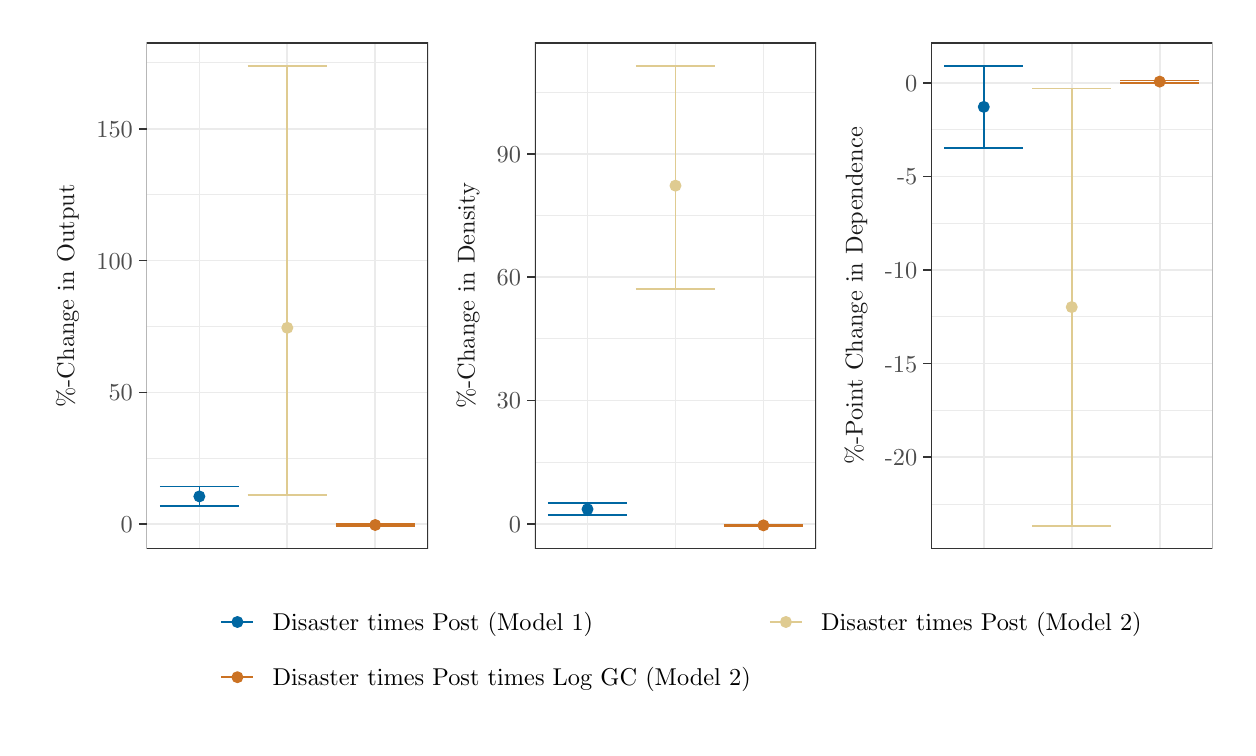
\begin{tikzpicture}[x=1pt,y=1pt]
\definecolor{fillColor}{RGB}{255,255,255}
\path[use as bounding box,fill=fillColor,fill opacity=0.00] (0,0) rectangle (433.62,252.94);
\begin{scope}
\path[clip] (  0.00,  0.00) rectangle (433.62,252.94);
\definecolor{drawColor}{RGB}{255,255,255}
\definecolor{fillColor}{RGB}{255,255,255}

\path[draw=drawColor,line width= 0.6pt,line join=round,line cap=round,fill=fillColor] (  0.00,  0.00) rectangle (433.62,252.94);
\end{scope}
\begin{scope}
\path[clip] ( 42.97, 64.66) rectangle (144.66,247.44);
\definecolor{fillColor}{RGB}{255,255,255}

\path[fill=fillColor] ( 42.97, 64.66) rectangle (144.66,247.44);
\definecolor{drawColor}{gray}{0.92}

\path[draw=drawColor,line width= 0.3pt,line join=round] ( 42.97, 97.31) --
	(144.66, 97.31);

\path[draw=drawColor,line width= 0.3pt,line join=round] ( 42.97,144.94) --
	(144.66,144.94);

\path[draw=drawColor,line width= 0.3pt,line join=round] ( 42.97,192.57) --
	(144.66,192.57);

\path[draw=drawColor,line width= 0.3pt,line join=round] ( 42.97,240.21) --
	(144.66,240.21);

\path[draw=drawColor,line width= 0.6pt,line join=round] ( 42.97, 73.49) --
	(144.66, 73.49);

\path[draw=drawColor,line width= 0.6pt,line join=round] ( 42.97,121.13) --
	(144.66,121.13);

\path[draw=drawColor,line width= 0.6pt,line join=round] ( 42.97,168.76) --
	(144.66,168.76);

\path[draw=drawColor,line width= 0.6pt,line join=round] ( 42.97,216.39) --
	(144.66,216.39);

\path[draw=drawColor,line width= 0.6pt,line join=round] ( 62.04, 64.66) --
	( 62.04,247.44);

\path[draw=drawColor,line width= 0.6pt,line join=round] ( 93.82, 64.66) --
	( 93.82,247.44);

\path[draw=drawColor,line width= 0.6pt,line join=round] (125.59, 64.66) --
	(125.59,247.44);
\definecolor{drawColor}{RGB}{0,103,162}
\definecolor{fillColor}{RGB}{0,103,162}

\path[draw=drawColor,line width= 0.4pt,line join=round,line cap=round,fill=fillColor] ( 62.04, 83.56) circle (  1.96);
\definecolor{drawColor}{RGB}{223,203,145}
\definecolor{fillColor}{RGB}{223,203,145}

\path[draw=drawColor,line width= 0.4pt,line join=round,line cap=round,fill=fillColor] ( 93.82,144.49) circle (  1.96);
\definecolor{drawColor}{RGB}{203,114,35}
\definecolor{fillColor}{RGB}{203,114,35}

\path[draw=drawColor,line width= 0.4pt,line join=round,line cap=round,fill=fillColor] (125.59, 73.23) circle (  1.96);
\definecolor{drawColor}{RGB}{0,103,162}

\path[draw=drawColor,line width= 0.6pt,line join=round] ( 47.74, 87.20) --
	( 76.34, 87.20);

\path[draw=drawColor,line width= 0.6pt,line join=round] ( 62.04, 87.20) --
	( 62.04, 80.05);

\path[draw=drawColor,line width= 0.6pt,line join=round] ( 47.74, 80.05) --
	( 76.34, 80.05);
\definecolor{drawColor}{RGB}{223,203,145}

\path[draw=drawColor,line width= 0.6pt,line join=round] ( 79.51,239.14) --
	(108.12,239.14);

\path[draw=drawColor,line width= 0.6pt,line join=round] ( 93.82,239.14) --
	( 93.82, 84.18);

\path[draw=drawColor,line width= 0.6pt,line join=round] ( 79.51, 84.18) --
	(108.12, 84.18);
\definecolor{drawColor}{RGB}{203,114,35}

\path[draw=drawColor,line width= 0.6pt,line join=round] (111.29, 73.49) --
	(139.89, 73.49);

\path[draw=drawColor,line width= 0.6pt,line join=round] (125.59, 73.49) --
	(125.59, 72.97);

\path[draw=drawColor,line width= 0.6pt,line join=round] (111.29, 72.97) --
	(139.89, 72.97);
\definecolor{drawColor}{gray}{0.20}

\path[draw=drawColor,line width= 0.6pt,line join=round,line cap=round] ( 42.97, 64.66) rectangle (144.66,247.44);
\end{scope}
\begin{scope}
\path[clip] (183.23, 64.66) rectangle (284.92,247.44);
\definecolor{fillColor}{RGB}{255,255,255}

\path[fill=fillColor] (183.23, 64.66) rectangle (284.92,247.44);
\definecolor{drawColor}{gray}{0.92}

\path[draw=drawColor,line width= 0.3pt,line join=round] (183.23, 95.90) --
	(284.92, 95.90);

\path[draw=drawColor,line width= 0.3pt,line join=round] (183.23,140.49) --
	(284.92,140.49);

\path[draw=drawColor,line width= 0.3pt,line join=round] (183.23,185.07) --
	(284.92,185.07);

\path[draw=drawColor,line width= 0.3pt,line join=round] (183.23,229.65) --
	(284.92,229.65);

\path[draw=drawColor,line width= 0.6pt,line join=round] (183.23, 73.61) --
	(284.92, 73.61);

\path[draw=drawColor,line width= 0.6pt,line join=round] (183.23,118.19) --
	(284.92,118.19);

\path[draw=drawColor,line width= 0.6pt,line join=round] (183.23,162.78) --
	(284.92,162.78);

\path[draw=drawColor,line width= 0.6pt,line join=round] (183.23,207.36) --
	(284.92,207.36);

\path[draw=drawColor,line width= 0.6pt,line join=round] (202.30, 64.66) --
	(202.30,247.44);

\path[draw=drawColor,line width= 0.6pt,line join=round] (234.08, 64.66) --
	(234.08,247.44);

\path[draw=drawColor,line width= 0.6pt,line join=round] (265.86, 64.66) --
	(265.86,247.44);
\definecolor{drawColor}{RGB}{0,103,162}
\definecolor{fillColor}{RGB}{0,103,162}

\path[draw=drawColor,line width= 0.4pt,line join=round,line cap=round,fill=fillColor] (202.30, 78.94) circle (  1.96);
\definecolor{drawColor}{RGB}{223,203,145}
\definecolor{fillColor}{RGB}{223,203,145}

\path[draw=drawColor,line width= 0.4pt,line join=round,line cap=round,fill=fillColor] (234.08,195.85) circle (  1.96);
\definecolor{drawColor}{RGB}{203,114,35}
\definecolor{fillColor}{RGB}{203,114,35}

\path[draw=drawColor,line width= 0.4pt,line join=round,line cap=round,fill=fillColor] (265.86, 73.10) circle (  1.96);
\definecolor{drawColor}{RGB}{0,103,162}

\path[draw=drawColor,line width= 0.6pt,line join=round] (188.00, 81.12) --
	(216.60, 81.12);

\path[draw=drawColor,line width= 0.6pt,line join=round] (202.30, 81.12) --
	(202.30, 76.79);

\path[draw=drawColor,line width= 0.6pt,line join=round] (188.00, 76.79) --
	(216.60, 76.79);
\definecolor{drawColor}{RGB}{223,203,145}

\path[draw=drawColor,line width= 0.6pt,line join=round] (219.78,239.14) --
	(248.38,239.14);

\path[draw=drawColor,line width= 0.6pt,line join=round] (234.08,239.14) --
	(234.08,158.53);

\path[draw=drawColor,line width= 0.6pt,line join=round] (219.78,158.53) --
	(248.38,158.53);
\definecolor{drawColor}{RGB}{203,114,35}

\path[draw=drawColor,line width= 0.6pt,line join=round] (251.56, 73.23) --
	(280.16, 73.23);

\path[draw=drawColor,line width= 0.6pt,line join=round] (265.86, 73.23) --
	(265.86, 72.97);

\path[draw=drawColor,line width= 0.6pt,line join=round] (251.56, 72.97) --
	(280.16, 72.97);
\definecolor{drawColor}{gray}{0.20}

\path[draw=drawColor,line width= 0.6pt,line join=round,line cap=round] (183.23, 64.66) rectangle (284.92,247.44);
\end{scope}
\begin{scope}
\path[clip] (326.43, 64.66) rectangle (428.12,247.44);
\definecolor{fillColor}{RGB}{255,255,255}

\path[fill=fillColor] (326.43, 64.66) rectangle (428.12,247.44);
\definecolor{drawColor}{gray}{0.92}

\path[draw=drawColor,line width= 0.3pt,line join=round] (326.43, 80.80) --
	(428.12, 80.80);

\path[draw=drawColor,line width= 0.3pt,line join=round] (326.43,114.62) --
	(428.12,114.62);

\path[draw=drawColor,line width= 0.3pt,line join=round] (326.43,148.45) --
	(428.12,148.45);

\path[draw=drawColor,line width= 0.3pt,line join=round] (326.43,182.27) --
	(428.12,182.27);

\path[draw=drawColor,line width= 0.3pt,line join=round] (326.43,216.10) --
	(428.12,216.10);

\path[draw=drawColor,line width= 0.6pt,line join=round] (326.43, 97.71) --
	(428.12, 97.71);

\path[draw=drawColor,line width= 0.6pt,line join=round] (326.43,131.53) --
	(428.12,131.53);

\path[draw=drawColor,line width= 0.6pt,line join=round] (326.43,165.36) --
	(428.12,165.36);

\path[draw=drawColor,line width= 0.6pt,line join=round] (326.43,199.19) --
	(428.12,199.19);

\path[draw=drawColor,line width= 0.6pt,line join=round] (326.43,233.01) --
	(428.12,233.01);

\path[draw=drawColor,line width= 0.6pt,line join=round] (345.49, 64.66) --
	(345.49,247.44);

\path[draw=drawColor,line width= 0.6pt,line join=round] (377.27, 64.66) --
	(377.27,247.44);

\path[draw=drawColor,line width= 0.6pt,line join=round] (409.05, 64.66) --
	(409.05,247.44);
\definecolor{drawColor}{RGB}{0,103,162}
\definecolor{fillColor}{RGB}{0,103,162}

\path[draw=drawColor,line width= 0.4pt,line join=round,line cap=round,fill=fillColor] (345.49,224.31) circle (  1.96);
\definecolor{drawColor}{RGB}{223,203,145}
\definecolor{fillColor}{RGB}{223,203,145}

\path[draw=drawColor,line width= 0.4pt,line join=round,line cap=round,fill=fillColor] (377.27,151.97) circle (  1.96);
\definecolor{drawColor}{RGB}{203,114,35}
\definecolor{fillColor}{RGB}{203,114,35}

\path[draw=drawColor,line width= 0.4pt,line join=round,line cap=round,fill=fillColor] (409.05,233.45) circle (  1.96);
\definecolor{drawColor}{RGB}{0,103,162}

\path[draw=drawColor,line width= 0.6pt,line join=round] (331.19,239.14) --
	(359.79,239.14);

\path[draw=drawColor,line width= 0.6pt,line join=round] (345.49,239.14) --
	(345.49,209.48);

\path[draw=drawColor,line width= 0.6pt,line join=round] (331.19,209.48) --
	(359.79,209.48);
\definecolor{drawColor}{RGB}{223,203,145}

\path[draw=drawColor,line width= 0.6pt,line join=round] (362.97,230.97) --
	(391.57,230.97);

\path[draw=drawColor,line width= 0.6pt,line join=round] (377.27,230.97) --
	(377.27, 72.97);

\path[draw=drawColor,line width= 0.6pt,line join=round] (362.97, 72.97) --
	(391.57, 72.97);
\definecolor{drawColor}{RGB}{203,114,35}

\path[draw=drawColor,line width= 0.6pt,line join=round] (394.75,233.86) --
	(423.35,233.86);

\path[draw=drawColor,line width= 0.6pt,line join=round] (409.05,233.86) --
	(409.05,233.04);

\path[draw=drawColor,line width= 0.6pt,line join=round] (394.75,233.04) --
	(423.35,233.04);
\definecolor{drawColor}{gray}{0.20}

\path[draw=drawColor,line width= 0.6pt,line join=round,line cap=round] (326.43, 64.66) rectangle (428.12,247.44);
\end{scope}
\begin{scope}
\path[clip] (290.42, 64.66) rectangle (307.00,247.44);
\definecolor{drawColor}{gray}{0.10}

\node[text=drawColor,rotate= 90.00,anchor=base,inner sep=0pt, outer sep=0pt, scale=  0.88] at (301.74,156.05) {\%-Point Change in Dependence};
\end{scope}
\begin{scope}
\path[clip] (150.16, 64.66) rectangle (166.73,247.44);
\definecolor{drawColor}{gray}{0.10}

\node[text=drawColor,rotate= 90.00,anchor=base,inner sep=0pt, outer sep=0pt, scale=  0.88] at (161.48,156.05) {\%-Change in Density};
\end{scope}
\begin{scope}
\path[clip] (  5.50, 64.66) rectangle ( 22.07,247.44);
\definecolor{drawColor}{gray}{0.10}

\node[text=drawColor,rotate= 90.00,anchor=base,inner sep=0pt, outer sep=0pt, scale=  0.88] at ( 16.82,156.05) {\%-Change in Output};
\end{scope}
\begin{scope}
\path[clip] (  0.00,  0.00) rectangle (433.62,252.94);
\definecolor{drawColor}{gray}{0.30}

\node[text=drawColor,anchor=base east,inner sep=0pt, outer sep=0pt, scale=  0.88] at (321.48, 94.68) {-20};

\node[text=drawColor,anchor=base east,inner sep=0pt, outer sep=0pt, scale=  0.88] at (321.48,128.50) {-15};

\node[text=drawColor,anchor=base east,inner sep=0pt, outer sep=0pt, scale=  0.88] at (321.48,162.33) {-10};

\node[text=drawColor,anchor=base east,inner sep=0pt, outer sep=0pt, scale=  0.88] at (321.48,196.15) {-5};

\node[text=drawColor,anchor=base east,inner sep=0pt, outer sep=0pt, scale=  0.88] at (321.48,229.98) {0};
\end{scope}
\begin{scope}
\path[clip] (  0.00,  0.00) rectangle (433.62,252.94);
\definecolor{drawColor}{gray}{0.20}

\path[draw=drawColor,line width= 0.6pt,line join=round] (323.68, 97.71) --
	(326.43, 97.71);

\path[draw=drawColor,line width= 0.6pt,line join=round] (323.68,131.53) --
	(326.43,131.53);

\path[draw=drawColor,line width= 0.6pt,line join=round] (323.68,165.36) --
	(326.43,165.36);

\path[draw=drawColor,line width= 0.6pt,line join=round] (323.68,199.19) --
	(326.43,199.19);

\path[draw=drawColor,line width= 0.6pt,line join=round] (323.68,233.01) --
	(326.43,233.01);
\end{scope}
\begin{scope}
\path[clip] (  0.00,  0.00) rectangle (433.62,252.94);
\definecolor{drawColor}{gray}{0.30}

\node[text=drawColor,anchor=base east,inner sep=0pt, outer sep=0pt, scale=  0.88] at (178.28, 70.58) {0};

\node[text=drawColor,anchor=base east,inner sep=0pt, outer sep=0pt, scale=  0.88] at (178.28,115.16) {30};

\node[text=drawColor,anchor=base east,inner sep=0pt, outer sep=0pt, scale=  0.88] at (178.28,159.75) {60};

\node[text=drawColor,anchor=base east,inner sep=0pt, outer sep=0pt, scale=  0.88] at (178.28,204.33) {90};
\end{scope}
\begin{scope}
\path[clip] (  0.00,  0.00) rectangle (433.62,252.94);
\definecolor{drawColor}{gray}{0.20}

\path[draw=drawColor,line width= 0.6pt,line join=round] (180.48, 73.61) --
	(183.23, 73.61);

\path[draw=drawColor,line width= 0.6pt,line join=round] (180.48,118.19) --
	(183.23,118.19);

\path[draw=drawColor,line width= 0.6pt,line join=round] (180.48,162.78) --
	(183.23,162.78);

\path[draw=drawColor,line width= 0.6pt,line join=round] (180.48,207.36) --
	(183.23,207.36);
\end{scope}
\begin{scope}
\path[clip] (  0.00,  0.00) rectangle (433.62,252.94);
\definecolor{drawColor}{gray}{0.30}

\node[text=drawColor,anchor=base east,inner sep=0pt, outer sep=0pt, scale=  0.88] at ( 38.02, 70.46) {0};

\node[text=drawColor,anchor=base east,inner sep=0pt, outer sep=0pt, scale=  0.88] at ( 38.02,118.09) {50};

\node[text=drawColor,anchor=base east,inner sep=0pt, outer sep=0pt, scale=  0.88] at ( 38.02,165.73) {100};

\node[text=drawColor,anchor=base east,inner sep=0pt, outer sep=0pt, scale=  0.88] at ( 38.02,213.36) {150};
\end{scope}
\begin{scope}
\path[clip] (  0.00,  0.00) rectangle (433.62,252.94);
\definecolor{drawColor}{gray}{0.20}

\path[draw=drawColor,line width= 0.6pt,line join=round] ( 40.22, 73.49) --
	( 42.97, 73.49);

\path[draw=drawColor,line width= 0.6pt,line join=round] ( 40.22,121.13) --
	( 42.97,121.13);

\path[draw=drawColor,line width= 0.6pt,line join=round] ( 40.22,168.76) --
	( 42.97,168.76);

\path[draw=drawColor,line width= 0.6pt,line join=round] ( 40.22,216.39) --
	( 42.97,216.39);
\end{scope}
\begin{scope}
\path[clip] (  0.00,  0.00) rectangle (433.62,252.94);
\definecolor{fillColor}{RGB}{255,255,255}

\path[fill=fillColor] ( 63.06,  5.50) rectangle (408.03, 50.91);
\end{scope}
\begin{scope}
\path[clip] (  0.00,  0.00) rectangle (433.62,252.94);
\definecolor{fillColor}{RGB}{255,255,255}

\path[fill=fillColor] ( 68.56, 30.95) rectangle ( 83.01, 45.41);
\end{scope}
\begin{scope}
\path[clip] (  0.00,  0.00) rectangle (433.62,252.94);
\definecolor{drawColor}{RGB}{0,103,162}
\definecolor{fillColor}{RGB}{0,103,162}

\path[draw=drawColor,line width= 0.4pt,line join=round,line cap=round,fill=fillColor] ( 75.79, 38.18) circle (  1.96);
\end{scope}
\begin{scope}
\path[clip] (  0.00,  0.00) rectangle (433.62,252.94);
\definecolor{drawColor}{RGB}{0,103,162}

\path[draw=drawColor,line width= 0.6pt,line join=round] ( 70.01, 38.18) -- ( 81.57, 38.18);
\end{scope}
\begin{scope}
\path[clip] (  0.00,  0.00) rectangle (433.62,252.94);
\definecolor{fillColor}{RGB}{255,255,255}

\path[fill=fillColor] (266.76, 30.95) rectangle (281.21, 45.41);
\end{scope}
\begin{scope}
\path[clip] (  0.00,  0.00) rectangle (433.62,252.94);
\definecolor{drawColor}{RGB}{223,203,145}
\definecolor{fillColor}{RGB}{223,203,145}

\path[draw=drawColor,line width= 0.4pt,line join=round,line cap=round,fill=fillColor] (273.99, 38.18) circle (  1.96);
\end{scope}
\begin{scope}
\path[clip] (  0.00,  0.00) rectangle (433.62,252.94);
\definecolor{drawColor}{RGB}{223,203,145}

\path[draw=drawColor,line width= 0.6pt,line join=round] (268.20, 38.18) -- (279.77, 38.18);
\end{scope}
\begin{scope}
\path[clip] (  0.00,  0.00) rectangle (433.62,252.94);
\definecolor{fillColor}{RGB}{255,255,255}

\path[fill=fillColor] ( 68.56, 11.00) rectangle ( 83.01, 25.45);
\end{scope}
\begin{scope}
\path[clip] (  0.00,  0.00) rectangle (433.62,252.94);
\definecolor{drawColor}{RGB}{203,114,35}
\definecolor{fillColor}{RGB}{203,114,35}

\path[draw=drawColor,line width= 0.4pt,line join=round,line cap=round,fill=fillColor] ( 75.79, 18.23) circle (  1.96);
\end{scope}
\begin{scope}
\path[clip] (  0.00,  0.00) rectangle (433.62,252.94);
\definecolor{drawColor}{RGB}{203,114,35}

\path[draw=drawColor,line width= 0.6pt,line join=round] ( 70.01, 18.23) -- ( 81.57, 18.23);
\end{scope}
\begin{scope}
\path[clip] (  0.00,  0.00) rectangle (433.62,252.94);
\definecolor{drawColor}{RGB}{0,0,0}

\node[text=drawColor,anchor=base west,inner sep=0pt, outer sep=0pt, scale=  0.88] at ( 88.51, 35.15) {Disaster times Post (Model 1)};
\end{scope}
\begin{scope}
\path[clip] (  0.00,  0.00) rectangle (433.62,252.94);
\definecolor{drawColor}{RGB}{0,0,0}

\node[text=drawColor,anchor=base west,inner sep=0pt, outer sep=0pt, scale=  0.88] at (286.71, 35.15) {Disaster times Post (Model 2)};
\end{scope}
\begin{scope}
\path[clip] (  0.00,  0.00) rectangle (433.62,252.94);
\definecolor{drawColor}{RGB}{0,0,0}

\node[text=drawColor,anchor=base west,inner sep=0pt, outer sep=0pt, scale=  0.88] at ( 88.51, 15.20) {Disaster times Post times Log GC (Model 2)};
\end{scope}
\end{tikzpicture}
